\chapter{激素对生殖的调控}\label{ch:g11:hormones-and-reproduction}

一位女性记录了一张图表：每天早晨的体温，
每月中旬有一次小幅升高；每二十八天左右一次出血。
若在实验室中每天测量她血液中的四种\omterm{def:g11:hormones-and-reproduction:hormone}{激素}，
会得到四条曲线，它们按固定顺序一次次升降，月复一月，
每一个峰值都引发下一个。男性的实验室图表则显示，
同样的\omterm{def:g11:hormones-and-reproduction:hormone}{激素}水平几乎保持恒定，日复一日。
两者的器官不同，但控制系统相同：脑中的一个中枢、
其下方的一个腺体、性腺，以及血液在两个方向上传递的信息。
本章将解读这些图表，
并说明对它们的理解如何使人们得以避孕，
或实现受孕。

\section{激素与反馈回路}

\begin{definition}[激素，反馈]\label{def:g11:hormones-and-reproduction:hormone}
\emph{激素}\index{激素}是由腺体分泌进入血液
的一种分子，通过远距离作用于带有其\emph{受体}的\omterm{def:g10:cells-common-unit:cell}{细胞}。
激素系统受\emph{反馈}\index{反馈}调节：链条末端产生的激素
反过来作用于链条起点处的腺体。
\emph{负反馈}——
产物抑制指令——使某一水平保持恒定；
\emph{正反馈}——产物增强指令——
则产生激增。
\end{definition}

\begin{proposition}[共同的链条]\label{prop:g11:hormones-and-reproduction:chain}
在两性中，同样的三级链条控制性腺。
脑中的一个中枢，即\emph{下丘脑}，将释放\omterm{def:g11:hormones-and-reproduction:hormone}{激素} GnRH 脉冲式地
分泌到通向其正下方\emph{垂体}的小血管中；
垂体随之向全身血液分泌两种\omterm{def:g11:hormones-and-reproduction:hormone}{激素}，
即\emph{LH}和\emph{FSH}；它们作用于性腺，
性腺产生配子和性\omterm{def:g11:hormones-and-reproduction:hormone}{激素}：睾丸产生睾酮，
卵巢产生雌\omterm{def:g11:hormones-and-reproduction:hormone}{激素}和孕酮。
性\omterm{def:g11:hormones-and-reproduction:hormone}{激素}作用于身体，
并反过来作用于下丘脑和垂体。
\end{proposition}
\admitted

\section{男性：水平恒定}

\begin{proposition}[睾丸的调控]\label{prop:g11:hormones-and-reproduction:male}
睾丸有两个部分。\emph{生精小管}受 FSH 和睾酮刺激，
自\omterm{prop:g11:becoming-male-female:puberty}{青春期}起持续产生精子，每天约一亿个。
小管之间的\omterm{def:g10:cells-common-unit:cell}{细胞}受 LH 刺激，
分泌\emph{睾酮}，睾酮维持生殖道、
第二性征和精子的产生。
睾酮抑制下丘脑和垂体：
睾酮升高时，GnRH、LH 和 FSH 下降，
睾丸分泌随之减少；睾酮降低时，它们则上升。
这种负\omterm{def:g11:hormones-and-reproduction:hormone}{反馈}使水平几乎保持恒定，
仅有每日的小幅波动，从\omterm{prop:g11:becoming-male-female:puberty}{青春期}直至老年。
\end{proposition}
\begin{proof}[证据]
去势动物的 LH 在数日内升高数倍；
注射睾酮后，LH 又降下来。
下丘脑损伤会使 LH、FSH 和睾酮同时消失；
脉冲式注射 GnRH 可使三者全部恢复，而持续输注 GnRH 则不能——
脉冲方式很重要。因其他原因接受睾酮治疗的男性，
其精子产量会下降：外源\omterm{def:g11:hormones-and-reproduction:hormone}{激素}
关闭了他们自身的垂体。
\end{proof}

\begin{omfigure}
\begin{tikzpicture}[font=\small, >=Stealth,
  b/.style={draw, rounded corners, align=center, text width=2.8cm, minimum height=1.0cm}]
  \node[b, fill=omDef!12] (h) at (0,3.2) {下丘脑};
  \node[b, fill=omDef!12] (p) at (0,1.6) {垂体};
  \node[b, fill=omProp!15] (t) at (0,0) {睾丸};
  \node[b, fill=omMeth!15, text width=3.6cm] (body) at (6.0,0) {精子产生；\\ 生殖道、\\ 第二性征};
  \draw[->, thick] (h) -- node[right] {GnRH（脉冲）} (p);
  \draw[->, thick] (p) -- node[right] {LH, FSH} (t);
  \draw[->, thick] (t) -- node[above] {睾酮} (body);
  \draw[->, thick, omThm, rounded corners=4pt] (t.west) -- (-2.3,0) -- (-2.3,3.2) -- (h.west);
  \node[omThm, anchor=east, align=right] at (-2.45,1.6) {睾酮 \\ 抑制};
  \draw[->, thick, omThm] (-2.3,1.6) -- (p.west);
  \node[omThm, font=\scriptsize] at (-0.7,0.35) {$-$};
\end{tikzpicture}

{\small 睾丸的调控。下丘脑驱动垂体，
垂体驱动睾丸，睾丸分泌的睾酮
同时抑制两者：这是一个使睾酮
保持近似恒定的负\omterm{def:g11:hormones-and-reproduction:hormone}{反馈}回路。}
\end{omfigure}

\section{女性：周期}

\begin{proposition}[卵巢周期]\label{prop:g11:hormones-and-reproduction:ovary}
从\omterm{prop:g11:becoming-male-female:puberty}{青春期}到绝经，卵巢运行一个约 28 天的周期。
\begin{itemize}
  \item \emph{卵泡期}（第 1--13 天）：在 FSH 作用下，卵泡
——一个被其营养\omterm{def:g10:cells-common-unit:cell}{细胞}包围的卵\omterm{def:g10:cells-common-unit:cell}{细胞}——生长，
        并分泌不断增加的\emph{雌\omterm{def:g11:hormones-and-reproduction:hormone}{激素}}。
  \item \emph{排卵}（第 14 天）：LH 的激增使成熟的
        卵泡破裂，释放其中的卵\omterm{def:g10:cells-common-unit:cell}{细胞}进入输卵管。
  \item \emph{黄体期}（第 15--28 天）：排卵后的卵泡
        变为\emph{黄体}，分泌\emph{孕酮}和雌\omterm{def:g11:hormones-and-reproduction:hormone}{激素}；
        若未开始妊娠，黄体约在十二天后退化，
        两种\omterm{def:g11:hormones-and-reproduction:hormone}{激素}随之下降，
        新的周期开始。
\end{itemize}
\end{proposition}
\admitted

\begin{omfigure}
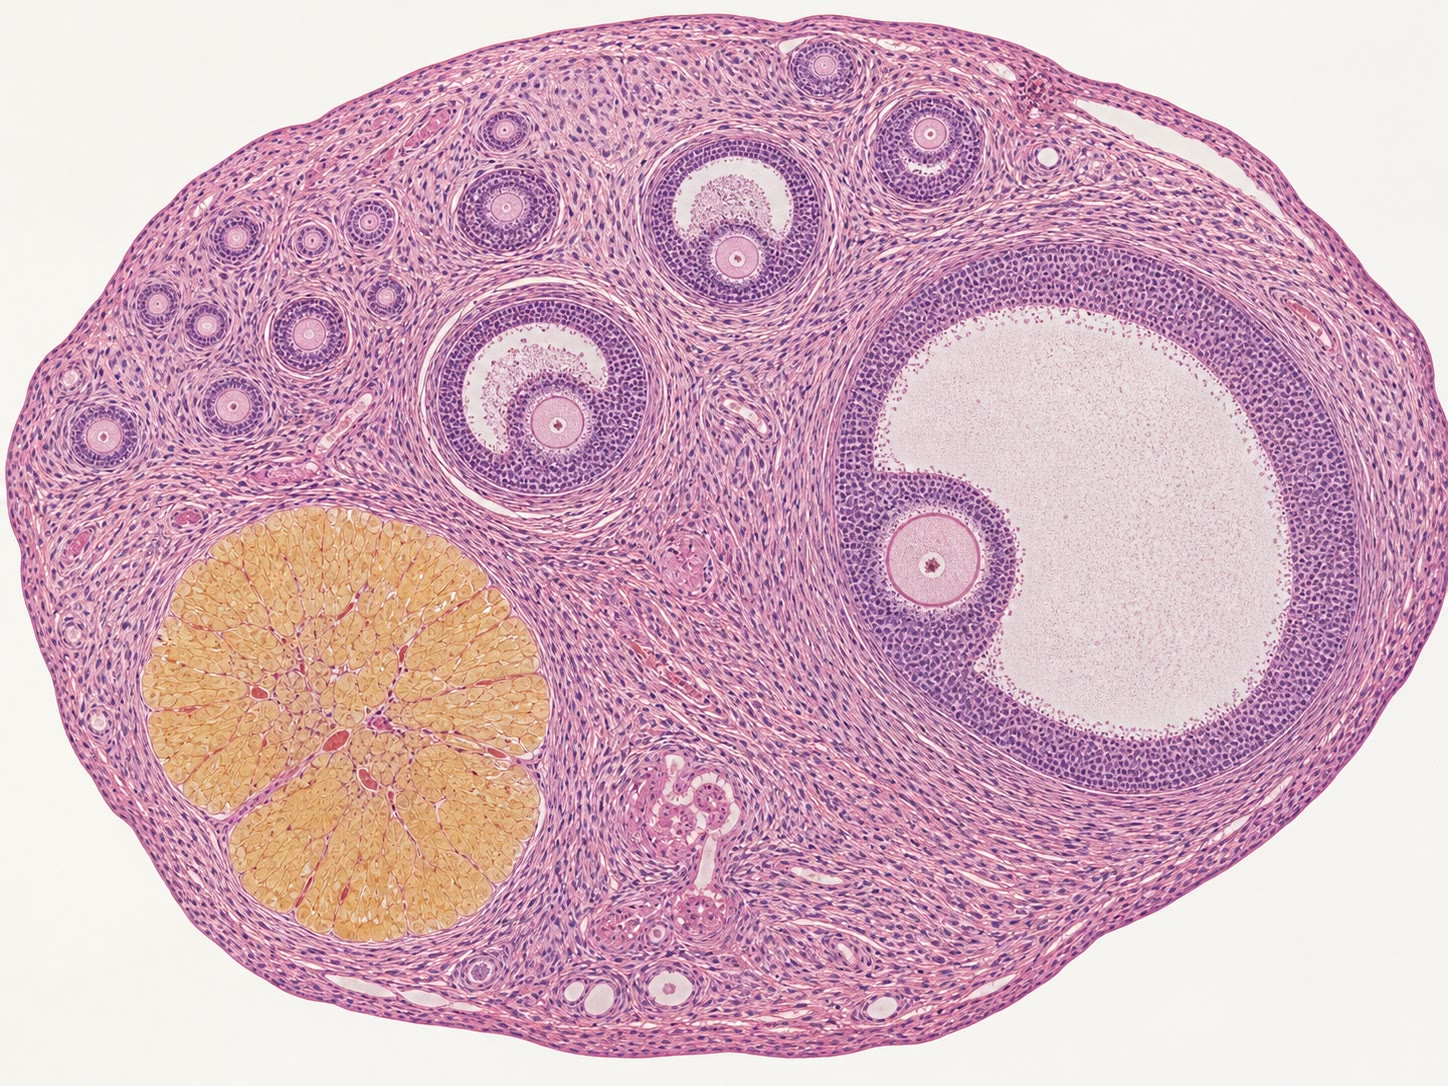
\includegraphics[width=0.56\linewidth]{images/book2/ai/g11-ovary-section.jpg}

{\small 卵巢切片：处于不同生长阶段的卵泡，
最大的一个内有充满液体的腔及其中的卵\omterm{def:g10:cells-common-unit:cell}{细胞}，
以及一个黄体——已排卵卵泡的残留物。}
\end{omfigure}

\begin{proposition}[子宫周期与反馈]\label{prop:g11:hormones-and-reproduction:uterus}
子宫内膜随卵巢\omterm{def:g11:hormones-and-reproduction:hormone}{激素}变化：雌\omterm{def:g11:hormones-and-reproduction:hormone}{激素}
使其在卵泡期增厚；孕酮使其
在黄体期转为分泌期，为接收胚胎做好准备；
周期末两者同时下降，使其剥落出血，
——\emph{月经}，即下一周期的第 1 至 5 天。\omterm{def:g11:hormones-and-reproduction:hormone}{反馈}
在周期中符号会改变：低水平和中等水平时，雌\omterm{def:g11:hormones-and-reproduction:hormone}{激素}
与孕酮抑制下丘脑和垂体（负\omterm{def:g11:hormones-and-reproduction:hormone}{反馈}）；
但成熟卵泡分泌的高水平雌\omterm{def:g11:hormones-and-reproduction:hormone}{激素}持续两天，
则\emph{刺激}它们（正\omterm{def:g11:hormones-and-reproduction:hormone}{反馈}），从而
引发触发排卵的 LH 峰。排卵后，
黄体分泌的孕酮恢复负\omterm{def:g11:hormones-and-reproduction:hormone}{反馈}，
不再出现第二次峰值。
\end{proposition}
\begin{proof}[证据]
每日血液测量给出下图曲线：LH
峰比雌\omterm{def:g11:hormones-and-reproduction:hormone}{激素}峰晚一天，比排卵早一天；
孕酮仅在排卵后出现。切除卵巢
会使 LH 和 FSH 升高，少量雌\omterm{def:g11:hormones-and-reproduction:hormone}{激素}使其降低；大剂量
且持续地在周期中期给予时可引发 LH 峰——\omterm{def:g11:hormones-and-reproduction:hormone}{反馈}的符号
随剂量而反转。若某女性的垂体不能
对雌\omterm{def:g11:hormones-and-reproduction:hormone}{激素}的上升作出反应，则无 LH 峰、不排卵，
尽管其卵泡仍会生长。
\end{proof}

\begin{omfigure}
\begin{tikzpicture}
\begin{axis}[
  width=0.92\linewidth, height=6.4cm,
  axis x line=bottom, axis y line=left,
  xmin=0, xmax=28, ymin=0, ymax=122,
  xlabel={周期中的天数}, ylabel={激素（占其最大值的 \%）},
  xlabel style={font=\small, at={(axis description cs:0.5,-0.1)}, anchor=north},
  ylabel style={font=\small},
  tick label style={font=\small}, xtick={0,7,14,21,28}, ytick={0,50,100},
  legend style={at={(0.5,-0.22)}, anchor=north, legend columns=4, font=\small, draw=none},
  clip=false,
]
\addplot[thick, omMeth, smooth] coordinates {(0,10) (4,15) (8,30) (11,70) (12,100) (13,80) (14,45) (16,35) (19,55) (22,60) (25,40) (28,10)};
\addplot[thick, omProp, smooth] coordinates {(0,3) (12,3) (14,5) (16,30) (19,70) (21,100) (23,90) (25,55) (27,15) (28,5)};
\addplot[thick, omThm] coordinates {(0,15) (11,18) (12,35) (13,100) (14,60) (15,15) (28,12)};
\addplot[thick, omDef, dashed] coordinates {(0,45) (4,40) (9,30) (12,35) (13,70) (14,45) (15,20) (28,25)};
\draw[dashed, gray] (axis cs:14,0) -- (axis cs:14,113);
\node[font=\small, anchor=south] at (axis cs:14,113) {排卵};
\draw[<->, gray] (axis cs:0.3,104) -- (axis cs:13.7,104);
\node[font=\scriptsize, anchor=south] at (axis cs:7,105) {卵泡期};
\draw[<->, gray] (axis cs:14.3,104) -- (axis cs:27.7,104);
\node[font=\scriptsize, anchor=south] at (axis cs:21,105) {黄体期};
\legend{雌激素, 孕酮, LH, FSH}
\end{axis}
\end{tikzpicture}

{\small 一个周期内的\omterm{def:g11:hormones-and-reproduction:hormone}{激素}。雌\omterm{def:g11:hormones-and-reproduction:hormone}{激素}随卵泡生长而升高，
于第 12 天达峰值；LH 峰随后于第 13 天出现，
排卵于第 14 天；来自黄体的孕酮主导后半段，
并在末尾下降，引发月经。}
\end{omfigure}

\begin{omfigure}
\begin{tikzpicture}[font=\small, >=Stealth,
  b/.style={draw, rounded corners, align=center, text width=2.8cm, minimum height=1.0cm}]
  \node[b, fill=omDef!12] (h) at (0,3.2) {下丘脑};
  \node[b, fill=omDef!12] (p) at (0,1.6) {垂体};
  \node[b, fill=omProp!15] (o) at (0,0) {卵巢};
  \node[b, fill=omMeth!15, text width=3.4cm] (u) at (6.4,0) {子宫内膜：\\ 增厚，随后 \\ 为胚胎做好准备};
  \draw[->, thick] (h) -- node[right] {GnRH} (p);
  \draw[->, thick] (p) -- node[right] {FSH、LH} (o);
  \draw[->, thick] (o) -- node[above, align=center] {雌激素，\\ 孕酮} (u);
  \draw[->, thick, omThm, rounded corners=4pt] (o.west) -- (-2.3,0) -- (-2.3,3.2) -- (h.west);
  \node[omThm, anchor=east, align=right, text width=2.6cm] at (-2.45,0.9) {低或中等水平抑制 $(-)$};
  \draw[->, thick, omThm] (-2.3,1.6) -- (p.west);
  \draw[->, thick, omMeth!70!black] (o.north west) .. controls (-2.0,0.9) and (-2.0,2.3) .. (h.south west);
  \node[omMeth!70!black, font=\scriptsize, anchor=east, align=right, text width=2.4cm] at (-2.45,2.7) {连续两天的高雌激素刺激 $(+)$：LH 峰};
\end{tikzpicture}

{\small 卵巢的调控。与雄性的调控链相同，只是
\omterm{def:g11:hormones-and-reproduction:hormone}{反馈}符号会改变：大部分时间为负\omterm{def:g11:hormones-and-reproduction:hormone}{反馈}，两天雌\omterm{def:g11:hormones-and-reproduction:hormone}{激素}峰值期间为正\omterm{def:g11:hormones-and-reproduction:hormone}{反馈}，
由此触发 LH 峰与排卵。}
\end{omfigure}

\begin{method}[读懂周期图]\label{met:g11:hormones-and-reproduction:read}
\begin{enumerate}
  \item 找出 LH 峰值：排卵发生于其后一天；卵泡期
        指峰前的全部时段，黄体期
        指峰后的全部时段。
  \item 检查顺序：雌\omterm{def:g11:hormones-and-reproduction:hormone}{激素}峰、LH 峰、
        排卵、孕酮。顺序错误的曲线说明
        存在异常。
  \item 计数：黄体期在每位女性中都接近 14 天；
        周期长度随卵泡期而变化。排卵
        因此发生在下次月经前 14 天，而非
        上次月经后 14 天。
  \item 分析某种药物或损伤时，先问它增加或去除了哪种\omterm{def:g11:hormones-and-reproduction:hormone}{激素}，
        再看\omterm{def:g11:hormones-and-reproduction:hormone}{反馈}随后对其他\omterm{def:g11:hormones-and-reproduction:hormone}{激素}产生什么影响。
\end{enumerate}
\end{method}

\section{选择：避孕}

\begin{proposition}[激素避孕]\label{prop:g11:hormones-and-reproduction:contraception}
复方避孕药每天提供少量雌\omterm{def:g11:hormones-and-reproduction:hormone}{激素}
及一种类孕酮分子。在此剂量下，\omterm{def:g11:hormones-and-reproduction:hormone}{反馈}
始终为负\omterm{def:g11:hormones-and-reproduction:hormone}{反馈}：FSH 保持较低水平，没有卵泡成熟，无雌\omterm{def:g11:hormones-and-reproduction:hormone}{激素}峰，
不出现 LH 峰，也不排卵。子宫内膜
保持较薄，宫颈黏液保持较稠，二者构成两道屏障。
停服一周，\omterm{def:g11:hormones-and-reproduction:hormone}{激素}下降，子宫内膜
出血。其他方法作用于其他环节：宫内铜环
阻止受精与着床；紧急避孕药在性交后
数日内服用，可延迟排卵；避孕套阻止
配子相遇，并且是唯一同时能阻止
性传播感染的方法。
\end{proposition}
\admitted

\begin{example}[读懂避孕药的效果]\label{ex:g11:hormones-and-reproduction:pill}
在一名服用避孕药的女性的图表上，四条曲线都是平的：
雌\omterm{def:g11:hormones-and-reproduction:hormone}{激素}和孕酮维持在避孕药所提供的低而稳定的水平，
LH 和 FSH 低于各自周期中的最低值，全程没有峰值。
若在一盒药的前几天漏服，FSH 便会逃逸：一个
卵泡可能开始发育，其余的也可能随之发育。避孕药之所以有效，
是因为\omterm{def:g11:hormones-and-reproduction:hormone}{反馈}在起作用；漏服的一片药，就是\omterm{def:g11:hormones-and-reproduction:hormone}{反馈}上的一个缺口。
\end{example}

\section{获得：辅助生殖}

\begin{proposition}[未能怀孕时]\label{prop:g11:hormones-and-reproduction:art}
约每七对夫妇中有一对，在尝试怀孕一年后前来就诊。病因
常由多种因素共同造成：排卵缺失或不规律、输卵管堵塞、精子过少，
或精子无法活动，另有约三分之一的病例查不出明确原因。
治疗方法遵循生物学原理：
\begin{itemize}
  \item \emph{排卵诱导}：注射 FSH，或服用一种能阻断雌\omterm{def:g11:hormones-and-reproduction:hormone}{激素}负\omterm{def:g11:hormones-and-reproduction:hormone}{反馈}的药物，
        使卵泡成熟；
        随后注射类 LH 药物，在选定的时刻诱发排卵；
  \item \emph{人工授精}：于排卵时将处理过的精子
        送入子宫；
  \item \emph{体外受精}：促排卵后，
        用针从卵巢中取出卵子，并在培养皿中使其受精
——必要时向每个卵子注入一个精子——并
        在三至五天后将一枚或两枚胚胎
        植入子宫。约每三到四次尝试中有一次
        成功分娩；其余的可用冷冻胚胎再行尝试。
\end{itemize}
自然生殖链条中每一个失效的环节，
都由相应的干预手段取代。
\end{proposition}
\admitted

\begin{example}[一次尝试中的数字]\label{ex:g11:hormones-and-reproduction:ivf}
促排可获得 10 个卵子，其中 8 个成熟，5 个受精，3 个发育至
五日阶段；移植 1 个，冷冻 2 个。移植成功
率约为三分之一；若再加上两个冷冻胚胎，一次取卵
后获得分娩的概率升至约 60\%。
自 1978 年以来，该技术已使数百万名儿童出生；它也引发了
一些问题——关于未被使用的胚胎、父母的年龄，
以及可被挑选的内容——生物学无法回答这些问题。
\end{example}

\begin{remark}[相互交汇的两个系统]\label{rem:g11:hormones-and-reproduction:brain}
本章的\omterm{def:g11:hormones-and-reproduction:hormone}{激素}调控性腺与身体，但在人类身上，它们
并不像在许多动物中那样支配性行为；在那些动物中，交配与卵巢周期相关。
人类的性活动
在很大程度上独立于周期，并取决于
大脑中负责欲望、快感与依恋的系统——即与其他动机共用的奖赏回路——
以及个人的经历，
文化与选择。生殖与性彼此交叠，却并非同一回事，
\omterm{def:g11:hormones-and-reproduction:hormone}{激素}只调控前者。
\end{remark}

\section{练习}

\begin{exercise}[$\star$]\label{exo:g11:hormones-and-reproduction:1}
定义\omterm{def:g11:hormones-and-reproduction:hormone}{激素}和\omterm{def:g11:hormones-and-reproduction:hormone}{反馈}，并区分负\omterm{def:g11:hormones-and-reproduction:hormone}{反馈}
与正\omterm{def:g11:hormones-and-reproduction:hormone}{反馈}。
\end{exercise}

\begin{exercise}[$\star$]\label{exo:g11:hormones-and-reproduction:2}
写出调控性腺的三级调控链条，
并指出各级分泌的\omterm{def:g11:hormones-and-reproduction:hormone}{激素}。
\end{exercise}

\begin{exercise}[$\star$]\label{exo:g11:hormones-and-reproduction:3}
睾丸的两个部分分别是什么，
各自产生什么物质？
\end{exercise}

\begin{exercise}[$\star$]\label{exo:g11:hormones-and-reproduction:4}
列出卵巢周期各时期及其对应的\omterm{def:g11:hormones-and-reproduction:hormone}{激素}。
\end{exercise}

\begin{exercise}[$\star$]\label{exo:g11:hormones-and-reproduction:5}
月经是由什么引起的？
\end{exercise}

\begin{exercise}[$\star\star$]\label{exo:g11:hormones-and-reproduction:6}
根据周期图，求出雌\omterm{def:g11:hormones-and-reproduction:hormone}{激素}峰值、LH 峰值、
排卵及孕酮峰值所在的日期。
\end{exercise}

\begin{exercise}[$\star\star$]\label{exo:g11:hormones-and-reproduction:7}
解释去势为何会使 LH 升高，
以及注射睾酮为何又使其降低。
\end{exercise}

\begin{exercise}[$\star\star$]\label{exo:g11:hormones-and-reproduction:8}
解释为什么第 12 天的雌\omterm{def:g11:hormones-and-reproduction:hormone}{激素}峰值会引发 LH 激增，
而第 20 天的雌\omterm{def:g11:hormones-and-reproduction:hormone}{激素}却不会。
\end{exercise}

\begin{exercise}[$\star\star$]\label{exo:g11:hormones-and-reproduction:9}
某女性的周期为 35 天。她在哪一天排卵？
请说明理由。
\end{exercise}

\begin{exercise}[$\star\star$]\label{exo:g11:hormones-and-reproduction:10}
利用\omterm{def:g11:hormones-and-reproduction:hormone}{反馈}的正负性，解释复方避孕药如何
阻止排卵。
\end{exercise}

\begin{exercise}[$\star\star$]\label{exo:g11:hormones-and-reproduction:11}
一名为健美而服用睾酮的男子发现，其睾丸萎缩，
精子数量下降。请解释原因。
\end{exercise}

\begin{exercise}[$\star\star\star$]\label{exo:g11:hormones-and-reproduction:12}
某药物会阻断下丘脑的雌\omterm{def:g11:hormones-and-reproduction:hormone}{激素}受体。预测
它对 FSH、卵泡生长及排卵的影响，并说明
该药物为何可用于治疗部分不孕症。
\end{exercise}

\begin{exercise}[$\star\star\star$]\label{exo:g11:hormones-and-reproduction:13}
某女性的图表显示雌\omterm{def:g11:hormones-and-reproduction:hormone}{激素}出现峰值，但没有 LH 峰值，也没有孕酮。
请找出该调节链中的缺陷，并提出治疗方案。
\end{exercise}

\begin{exercise}[$\star\star\star$]\label{exo:g11:hormones-and-reproduction:14}
怀孕期间，胚胎组织分泌一种类 LH \omterm{def:g11:hormones-and-reproduction:hormone}{激素}，
使黄体保持活性。请解释该\omterm{def:g11:hormones-and-reproduction:hormone}{激素}为何能阻止月经
及之后的再次排卵，并说明验孕试验为何能检测到该\omterm{def:g11:hormones-and-reproduction:hormone}{激素}。
\end{exercise}

\begin{exercise}[$\star\star\star$]\label{exo:g11:hormones-and-reproduction:15}
一个体外受精周期收集到 12 个卵子，其中 60\% 受精，
受精卵中有 40\% 发育至第 5 天；每个移植的胚胎有 35\% 的
概率产生一次分娩。计算胚胎的期望数目，以及
在逐个移植、直至成功或胚胎用尽的情形下，
至少分娩一次的概率。
\end{exercise}

\section{问题：图表}

\begin{problem}[{周末问题——一名女性的周期，逐一绘制各激素的图表，
解读其中的反馈，受避孕药干扰，
并在周期失常时予以辅助}]
\label{pb:g11:hormones-and-reproduction:1}
在一个周期内每天采集血样。以下数值经取整，
表示各\omterm{def:g11:hormones-and-reproduction:hormone}{激素}占其最大值的百分比：

\begin{center}
\begin{tabular}{lccccccccc}
天 & 2 & 6 & 10 & 12 & 13 & 14 & 18 & 22 & 27 \\ \hline
雌\omterm{def:g11:hormones-and-reproduction:hormone}{激素} & 10 & 20 & 55 & 100 & 80 & 45 & 45 & 60 & 15 \\
LH & 15 & 15 & 20 & 35 & 100 & 60 & 15 & 15 & 12 \\
FSH & 45 & 35 & 30 & 35 & 70 & 45 & 22 & 25 & 25 \\
孕酮 & 3 & 3 & 3 & 3 & 4 & 5 & 55 & 100 & 15 \\
\end{tabular}
\end{center}

\medskip
\noindent\textbf{第一部分——读图。}
\begin{enumerate}
  \item 排卵发生在哪一天？请根据
        两种\omterm{def:g11:hormones-and-reproduction:hormone}{激素}加以说明。
  \item 写出卵泡期与黄体期，并给出各期长度。
  \item 卵巢的哪一结构分泌第 10 天的雌\omterm{def:g11:hormones-and-reproduction:hormone}{激素}？第 22 天的呢？
        第 22 天的孕酮由哪一结构分泌？
  \item 描述第 6 天、第 22 天和第 28 天子宫内膜的状态。
  \item 为何 FSH 在周期开始时最高，
        而在黄体期最低？
\end{enumerate}

\medskip
\noindent\textbf{第二部分——\omterm{def:g11:hormones-and-reproduction:hormone}{反馈}调节。}
\begin{enumerate}[resume]
  \item 第 2 至第 10 天之间，雌\omterm{def:g11:hormones-and-reproduction:hormone}{激素}上升，而 FSH 下降，
        起作用的是哪种\omterm{def:g11:hormones-and-reproduction:hormone}{反馈}？请予以解释。
  \item 第 12 至第 13 天之间，雌\omterm{def:g11:hormones-and-reproduction:hormone}{激素}处于峰值，LH
        升至原来的七倍。这是哪种\omterm{def:g11:hormones-and-reproduction:hormone}{反馈}？雌\omterm{def:g11:hormones-and-reproduction:hormone}{激素}水平
        需满足怎样的条件，该\omterm{def:g11:hormones-and-reproduction:hormone}{反馈}才能发生？
  \item 第 18 至第 27 天之间，雌\omterm{def:g11:hormones-and-reproduction:hormone}{激素}水平适中，孕酮
        水平较高，LH 水平较低。这是哪种\omterm{def:g11:hormones-and-reproduction:hormone}{反馈}？为何不再
        出现第二次 LH 峰值？
  \item 黄体于第 26 天退化。预测第 28 天的\omterm{def:g11:hormones-and-reproduction:hormone}{激素}水平
        及随后发生的情况。
  \item 解释该周期为何能自行重启：哪一\omterm{def:g11:hormones-and-reproduction:hormone}{激素}在第 1 天的
        升高启动了下一个卵泡？
\end{enumerate}

\medskip
\noindent\textbf{第三部分——避孕药。}
同一女性连续一个月服用复方避孕药，该药
每天提供雌\omterm{def:g11:hormones-and-reproduction:hormone}{激素}，其量为最大值的 25\%；类孕酮\omterm{def:g11:hormones-and-reproduction:hormone}{激素}，
其量为最大值的 40\%。
\begin{enumerate}[resume]
  \item 预测整个月内 FSH 与 LH 的水平，以及
        卵泡的去向。
  \item 是否会出现雌\omterm{def:g11:hormones-and-reproduction:hormone}{激素}峰值？LH 峰值？排卵？
  \item 在停药的七天里，子宫内膜发生什么变化？
        为何这并不是真正的月经？
  \item 她在第 5 至第 8 天忘记服药。请逐步解释
        其中的风险。
  \item 解释为何单纯孕酮类避孕药，其水平足以维持
        负\omterm{def:g11:hormones-and-reproduction:hormone}{反馈}时，同样能阻止排卵。
\end{enumerate}

\medskip
\noindent\textbf{第四部分——调节链失效时。}
\begin{enumerate}[resume]
  \item 另一名女性的图表显示，FSH 与 LH 始终低于 10\%，
        雌\omterm{def:g11:hormones-and-reproduction:hormone}{激素}也低于 10\%。缺陷位于何处？
        应采用何种治疗恢复排卵，并通过何种途径实施？
  \item 第三名女性的图表正常，但其输卵管堵塞。
        \cref{prop:g11:hormones-and-reproduction:art}中的哪些步骤
        可替代受阻的步骤？
  \item 在体外受精中，于收集卵子前 36
        小时单次注射一剂类 LH \omterm{def:g11:hormones-and-reproduction:hormone}{激素}。请解释它模拟的是什么，
        以及为何时间须十分精确。
  \item 促排卵后有 10 个卵泡成熟，而非 1 个。
        请结合 FSH 解释，自然周期为何通常只使一个卵泡成熟。
  \item 请给出结论：图表中的排卵日、产生该排卵的\omterm{def:g11:hormones-and-reproduction:hormone}{反馈}的
        两个特征，
        以及避孕药抑制排卵的机制。
\end{enumerate}
\end{problem}
